% Needs graphicx, booktabs, makecell. Copy only the figures needed in the paper.
\begin{figure*}[!htbp]
\centering
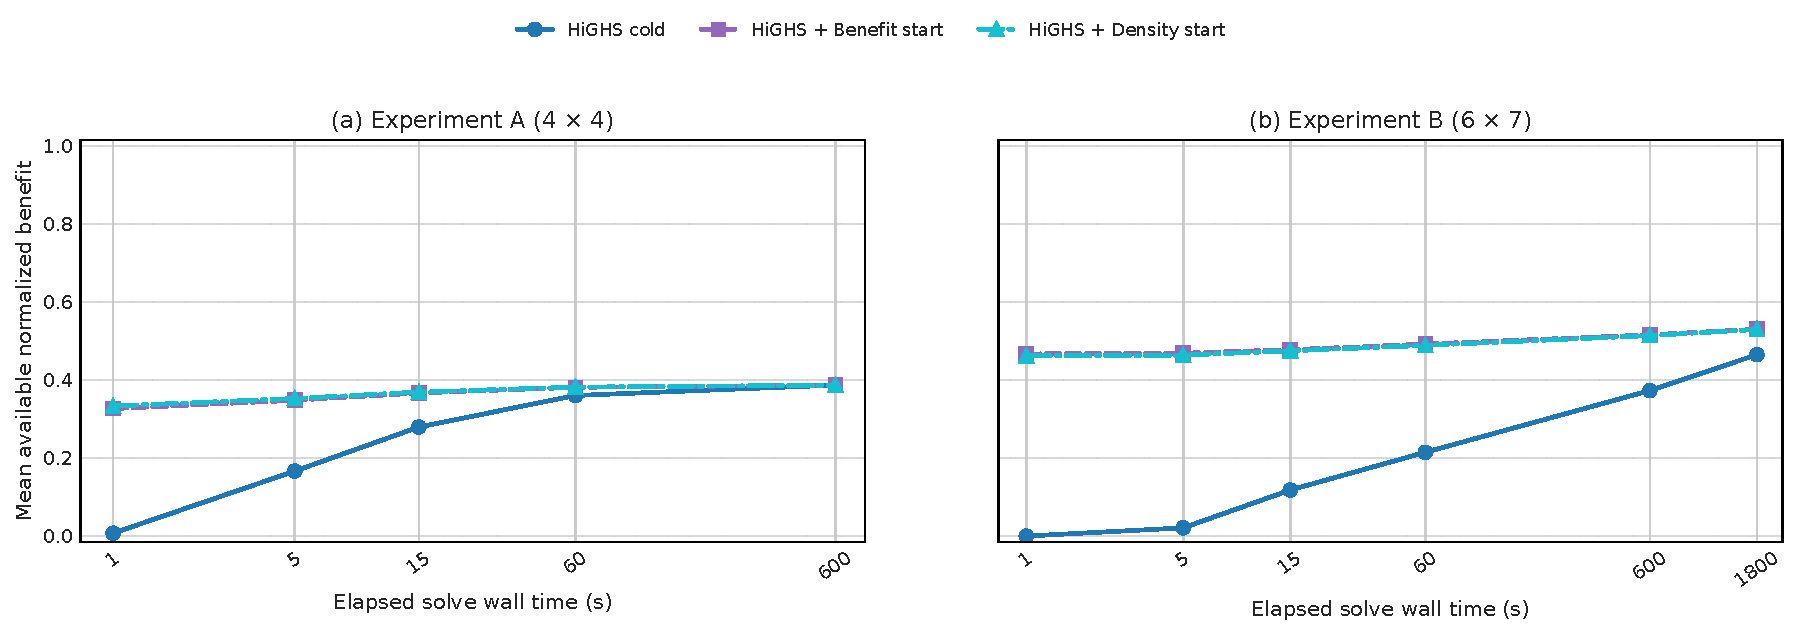
\includegraphics[width=\textwidth]{AB14_observed_available_benefit.pdf}
\caption{Available solution quality during a single long search: (a) Experiment A,
(b) Experiment B. Each curve averages all 150 instances. Validated greedy starts
are available at solve time zero; subsequent values use only incumbents observed
by the stated elapsed wall time. Cold searches without an observed incumbent
contribute idle value zero to this availability metric. Preparation is excluded.
The source search limits are 600 s in A and 1800 s in B. Lines connect the recorded
checkpoints and do not identify exact improvement times. These curves show
solution availability; they alone do not isolate the effect of injecting a start.}
\label{fig:AB-observed-quality}
\end{figure*}

% Recommended certification frontier when discussing actual solve-time budgets.
\begin{figure*}[!htbp]
\centering
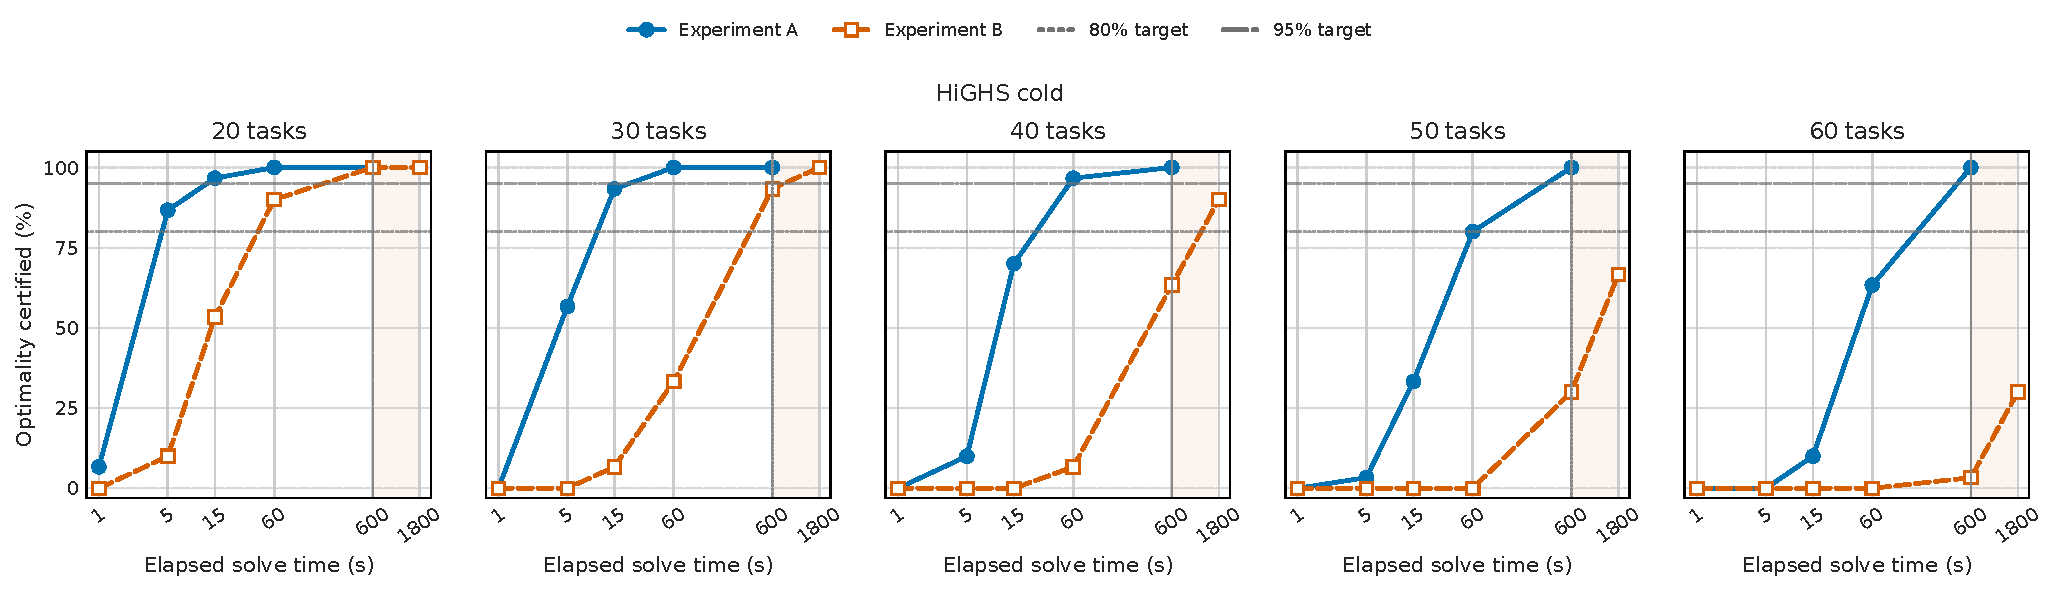
\includegraphics[width=\textwidth]{AB5_observed_certification_Cold.pdf}
\caption{Observed certification within a single long cold search per instance.
Each point counts the instances whose certified search had finished by the
stated elapsed solve time, out of 30 at that task count. Horizontal lines mark
80\% and 95\% targets. The shaded extension is tested only in Experiment B.
Preparation time is excluded. These checkpoints respect the recorded solve
clock and differ from the final outcomes of independent configured-limit runs.}
\label{fig:AB-observed-certification}
\end{figure*}

\begin{figure*}[!htbp]
\centering
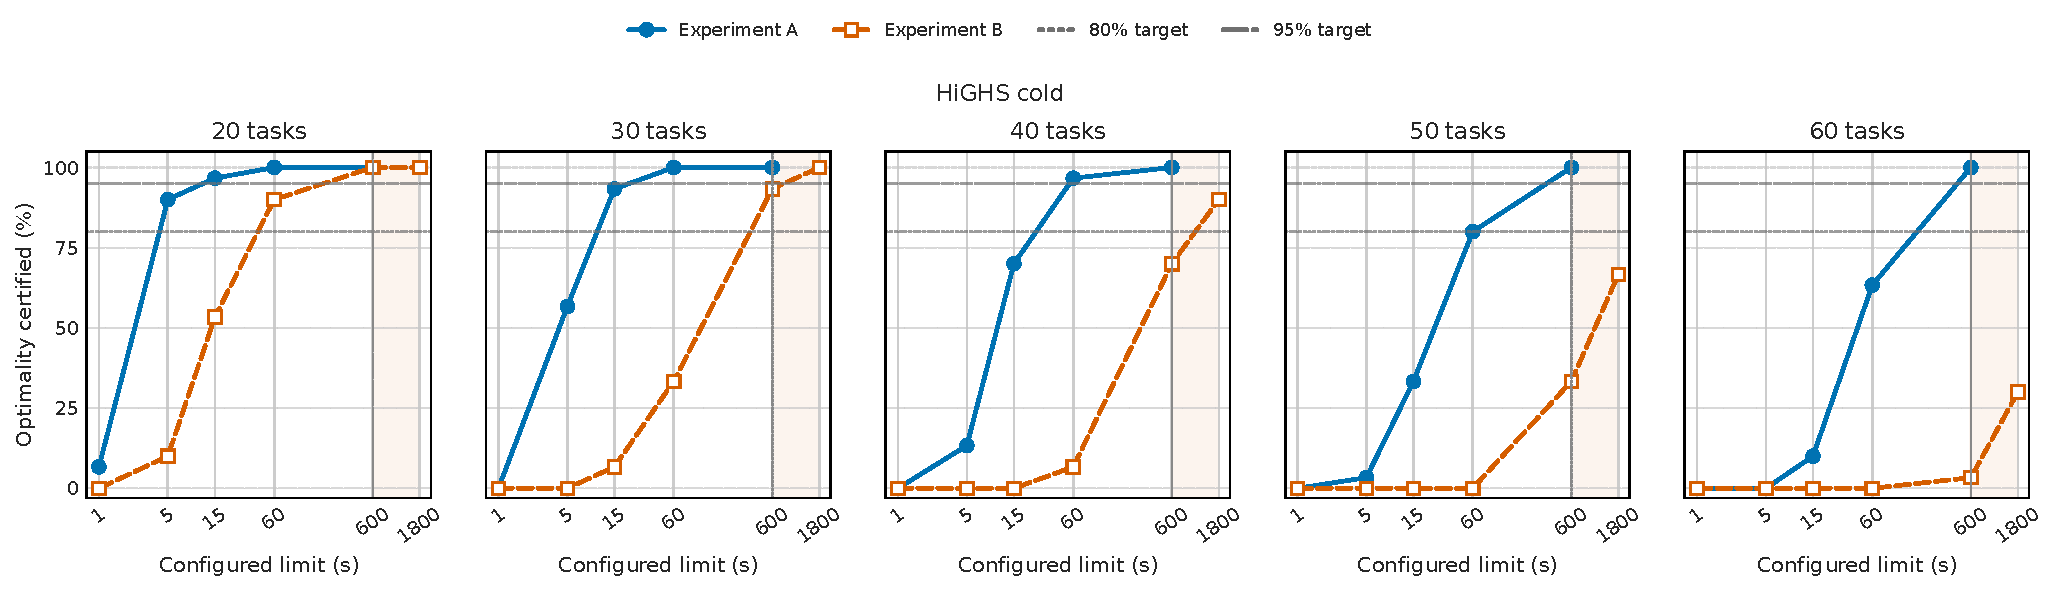
\includegraphics[width=\textwidth]{AB5_budget_certification_Cold.pdf}
\caption{Certification under configured solver limits, by task count, for cold
HiGHS searches in Experiments A and B. Each point summarizes 30 independent
instances. Horizontal lines mark the descriptive 80\% and 95\% targets. The
shaded region contains the 600--1800-s extension tested only in B. Configured
limits are not strict elapsed-time deadlines; actual times are reported separately.}
\label{fig:AB-certification-budget}
\end{figure*}

\begin{figure*}[!htbp]
\centering
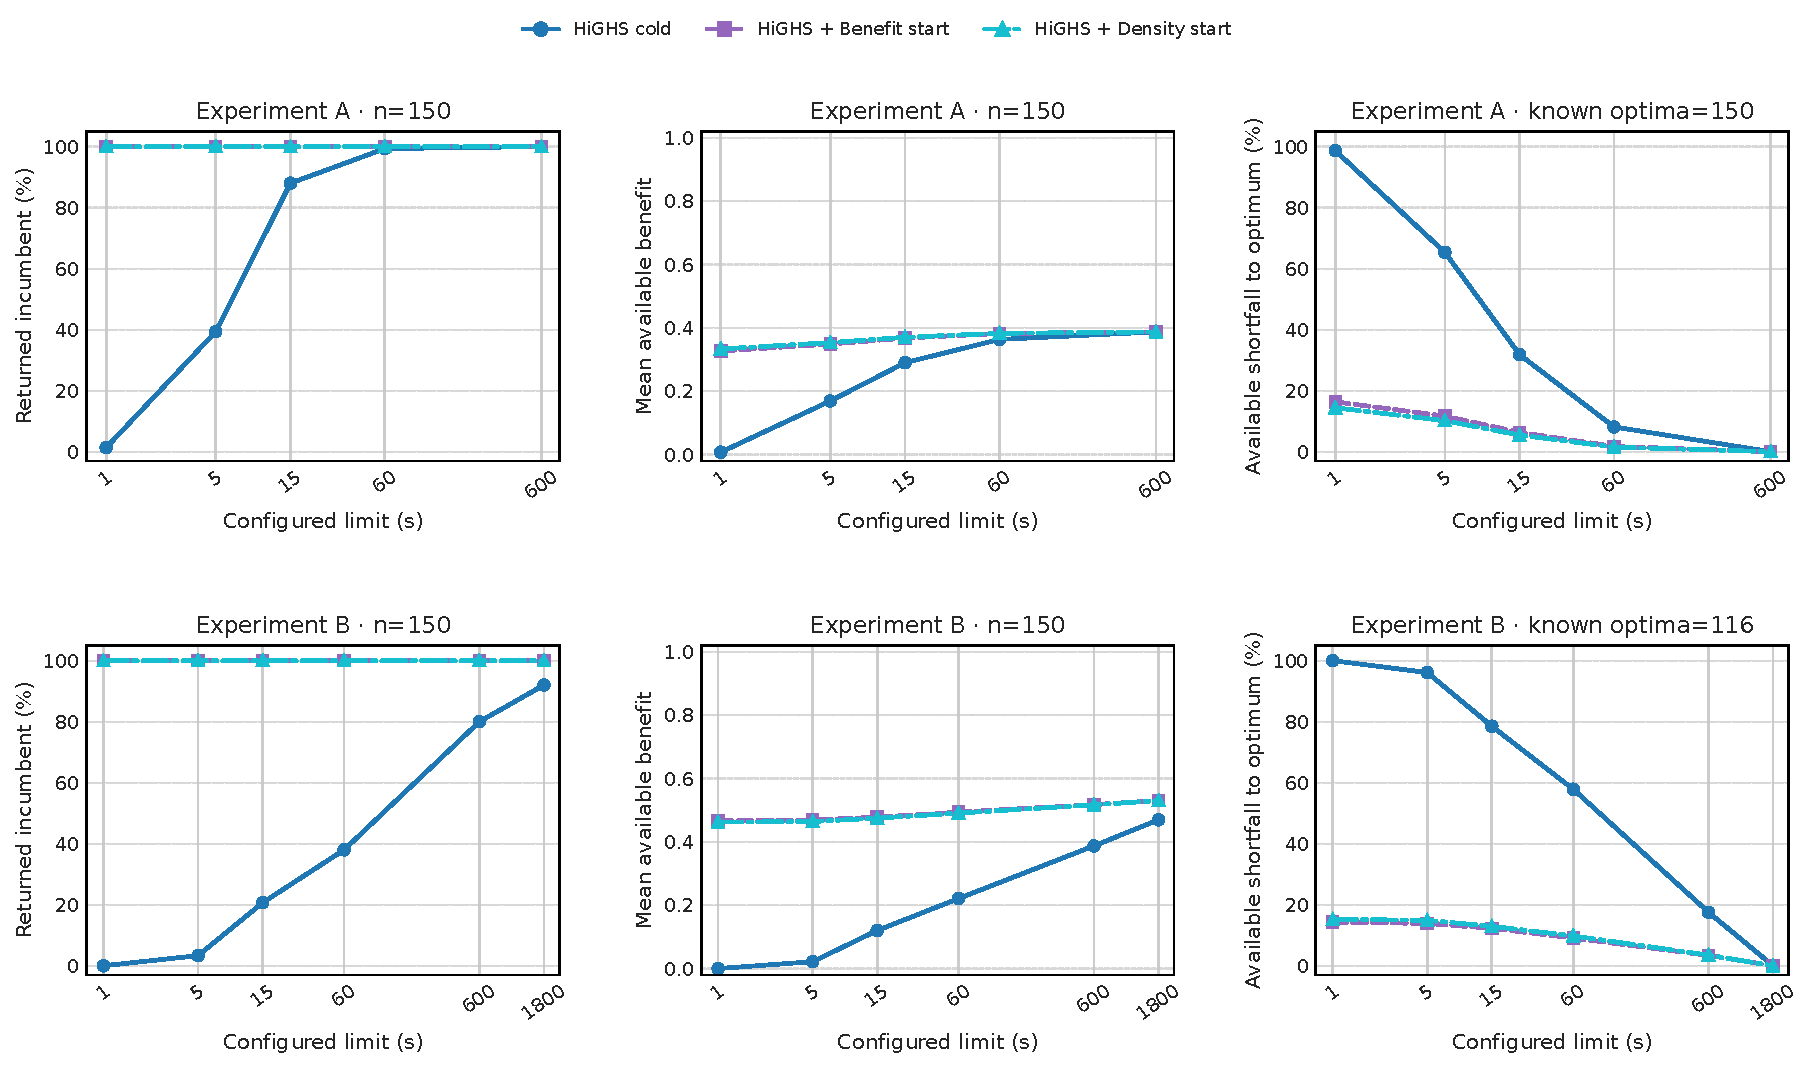
\includegraphics[width=\textwidth]{AB_budget_quality_dashboard.pdf}
\caption{Independent-run outcomes by configured limit. Rows correspond to
Experiments A and B. Returned-incumbent rates and mean available benefit use
all 150 instances. Available benefit assigns idle value zero separately when
no plan is returned; a validated start is available in each warm treatment.
The right panels average available-solution shortfalls over known certified
references only (150 in A, 116 in B), including idle values. These are different
statistics from conditional mean solver incumbents in Table~\ref{tab:AB-budget-status}.
Model and start preparation are excluded from the configured solver limit;
actual solve times may overrun that limit.}
\label{fig:AB-budget-quality}
\end{figure*}

% Optional supplementary attribution figure; use with the paired CSV counts.
\begin{figure*}[!htbp]
\centering
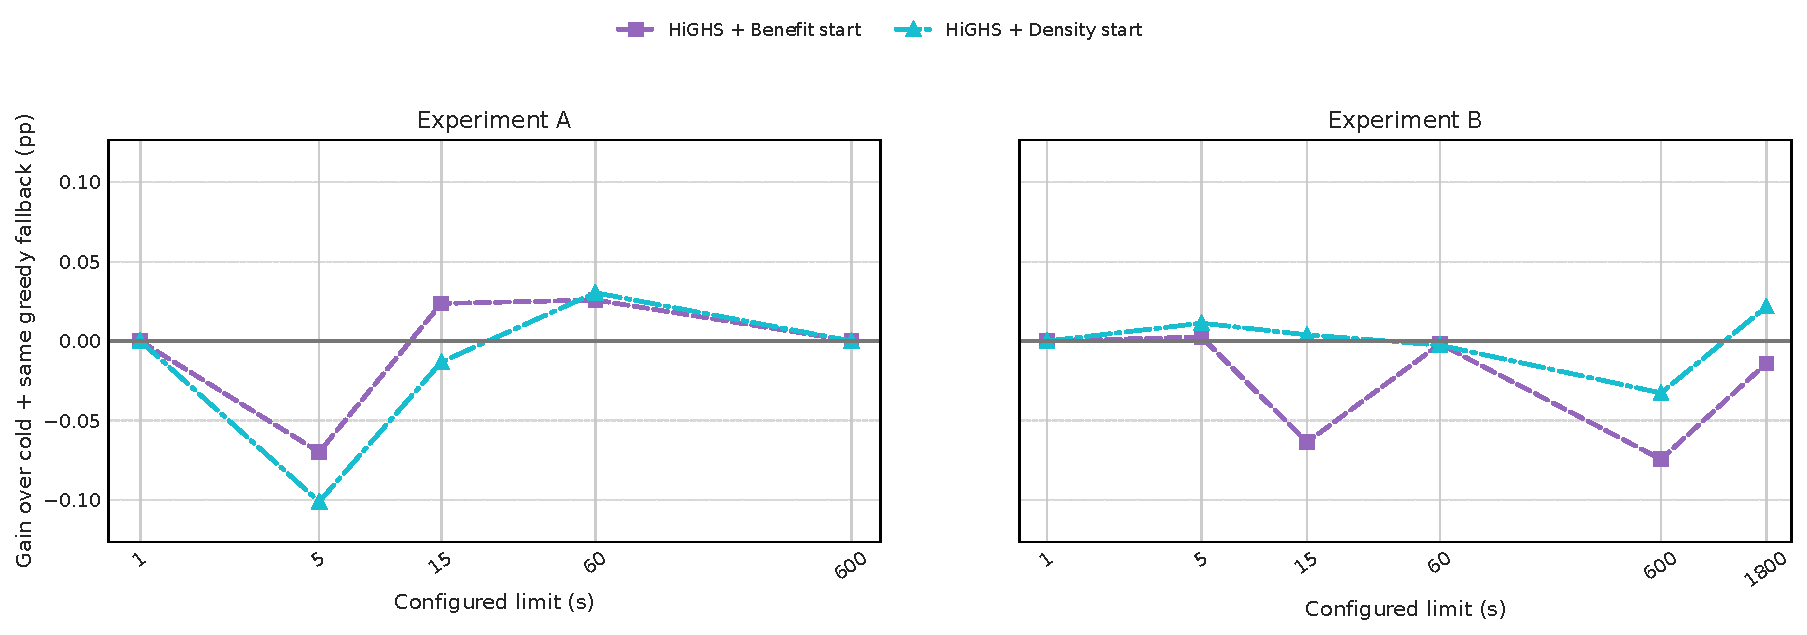
\includegraphics[width=\textwidth]{AB15_paired_injection_effect.pdf}
\caption{Paired mean incremental value of injecting a start rather than keeping
the same greedy as an external fallback. For each instance and configured limit,
the difference is $z_{\mathrm{warm}}-\max\{z_{\mathrm{cold}},z_{\mathrm{greedy}}\}$,
in percentage points of normalized benefit. Negative differences are retained.
All 150 instances are included in each experiment. Preparation and elapsed-time
overruns are reported separately; these are paired configured-limit comparisons.}
\label{fig:AB-injection-effect}
\end{figure*}
